\documentclass[11pt]{article}

\usepackage[margin=1in]{geometry}
\usepackage[T1]{fontenc}
\usepackage[utf8]{inputenc}
\usepackage{lmodern}
\usepackage{microtype}
\usepackage{amsmath,amssymb,amsthm,mathtools,bm}
\usepackage{graphicx}
\usepackage{booktabs}
\usepackage{xcolor}
\usepackage[numbers,sort&compress]{natbib}
\usepackage{algorithm}
\usepackage{algpseudocode}
\usepackage[colorlinks=true,linkcolor=blue!50!black,citecolor=blue!50!black,urlcolor=blue!50!black]{hyperref}
\usepackage[capitalise,nameinlink]{cleveref}

\newtheorem{theorem}{Theorem}
\newtheorem{proposition}[theorem]{Proposition}
\newtheorem{lemma}[theorem]{Lemma}
\newtheorem{corollary}[theorem]{Corollary}
\theoremstyle{definition}
\newtheorem{definition}[theorem]{Definition}
\newtheorem{problem}{Problem}
\theoremstyle{remark}
\newtheorem{remark}[theorem]{Remark}

\newcommand{\B}{\{0,1\}^n}
\newcommand{\R}{\mathbb{R}}
\newcommand{\E}{\mathcal{E}}
\newcommand{\X}{\mathcal{X}}
\newcommand{\simplex}{\Delta}
\newcommand{\hp}{\hat p}
\newcommand{\wh}[1]{\widehat{#1}}
\newcommand{\one}{\mathbf{1}}
\newcommand{\supp}{\operatorname{supp}}
\DeclareMathOperator*{\argmin}{arg\,min}

\title{Smoothing Bitstring Distributions:\\
From Frank--Wolfe to Walsh Filters, and Which Spectral Smoothers\\ Could Need a Quantum Computer}
\author{Lukas Thei{\ss}inger}
\date{October 2026}

\begin{document}
\maketitle

\begin{abstract}
A recent perspective by Belis et al.\ argues that spectral methods (learning, regularising or filtering the Fourier spectrum of a model) are central to machine learning and natural for quantum computers. Its motivating example is a generative model over bitstrings that smooths the empirical distribution by suppressing high-order Walsh coefficients. We revisit this example from first principles, starting from an optimisation viewpoint rather than a spectral one. We formalise smoothness by the Dirichlet energy on the Boolean hypercube and study two estimators. The first is penalised maximum likelihood, solved with a sparse, fully corrective Frank--Wolfe method. The second is $\ell_2$ denoising, which the hypercube Laplacian turns into a closed-form Walsh filter $1/(1+2\mu|S|)$.

We make five main observations.
(i) The Frank--Wolfe outer loop must not restart its step-size schedule. With a continuous clock, the split into outer and inner iterations becomes irrelevant whenever the support is stable. The KKT conditions give the optimum an obstacle-problem structure and an a-posteriori bound on its support size. Together these explain why, in the regimes we test, the support barely grows beyond the data.
(ii) The positivity constraint of the denoising problem is never active. $(I+\mu L)^{-1}$ is a strictly positive, doubly stochastic Markov kernel. It equals an exponentially weighted mixture of independent bit-flip channels and a geometric-length random walk, so the smoothed distribution can be sampled exactly in $O(n)$ time per draw and evaluated in $O(mn)$, for any $n$.
(iii) Using classical results on the Hamming association scheme, we recall which Walsh filters depending only on the Fourier level $|S|$ map distributions to distributions. These filters are exactly mixtures of ``flip $d$ uniformly random bits'' channels, so all of them are classically samplable, and the best one can be learned by a concave leave-one-out likelihood. Hard band-limiting always falls outside this class, and Gaussian decay in $|S|$ can too; on typical data such filters produce negative ``probabilities''.
(iv) Every positivity-preserving filter, isotropic or not, is a convolution with a noise distribution, an elementary fact of Fourier analysis on $\mathbb{Z}_2^n$. Applied to the quantum argument, it shows that classical hardness of probability-level smoothing therefore reduces exactly to hardness of sampling that noise. This points to a concrete quantum-relevant regime: noise from circuits such as IQP, mixed classically into the data. It also raises an open question about whether noise can be both local and hard to sample.
(v) Experiments up to $n=20$ (exact) and $n=100$ (sampling) confirm the theory, including a certified global optimum on all $2^{20}$ states. On held-out generalisation at $n=10$, with all kernel methods tuned by the same leave-one-out likelihood, the one-parameter heat kernel is as good as the learned positive isotropic filter on a Hamming-smooth target. On a parity-checksum target, the learned filter is the only smoother that beats the empirical distribution: it learns to flip only even numbers of bits and puts zero mass on invalid strings. In these experiments, penalised maximum likelihood barely moves mass off the observed strings.
\end{abstract}

% ------------------------------------------------------------------------------
\section{Introduction}

Belis et al.~\cite{belis2026spectral} put forward a research programme for quantum machine learning that starts from the question ``why quantum?''. Their answer is that many successful learning methods are, at heart, \emph{spectral}: they shape the Fourier spectrum of a model. Examples are the spectral bias of neural networks~\cite{rahaman2019spectral}, stationary kernels acting as Fourier filters, and convolutions. Quantum computers, in turn, can apply Fourier transforms over many groups efficiently. Their first and most concrete example is learning a distribution over bitstrings by smoothing the empirical distribution in the Walsh--Fourier domain. They also note (their Sec.~II.5) that one particular filter, $(1-2\theta)^{|S|}$, is just a classical kernel density estimator and is therefore dequantisable.

This paper works through that example from the point of view of someone trained in machine learning rather than signal processing. We write down a smoothness-regularised objective, try to optimise it, and only then discover that the problem is spectral. This route is longer, but it exposes several facts that the purely spectral presentation hides:

\begin{enumerate}
\item \textbf{Optimisation (\cref{sec:p1}).} Penalised maximum likelihood with a Dirichlet-energy regulariser is a convex problem on the simplex. A sparse, fully corrective Frank--Wolfe (FW) method solves it without materialising $2^n$ numbers. One implementation detail matters a lot: if the inner step-size schedule restarts at every outer iteration, the outer loop becomes a hidden restart heuristic (\cref{prop:clock}). The KKT conditions show that, off the data, the optimum solves a discrete obstacle problem, and they give an a-posteriori bound on its support size (\cref{prop:support}). This does not guarantee sparsity in general: for $n=1$ the optimum can put a third of its mass on the unseen string. But it explains why, in the regimes of our experiments, support discovery saturates almost immediately.

\item \textbf{The denoising view (\cref{sec:p2}).} Replacing the likelihood by an $\ell_2$ data term gives the closed form $p=(I+\mu L)^{-1}\hp$, where $L$ is the hypercube Laplacian. In the Walsh basis this is the filter $1/(1+2\mu|S|)$. We show that the simplex constraint is automatically satisfied (\cref{thm:p2}), which answers the question left open in the blog post this paper grew out of. We also give two exact $O(n)$ samplers and a closed-form, numerically exact density.

\item \textbf{Which filters are distributions? (\cref{sec:filters}).} Isotropic filters, those depending only on $|S|$, map distributions to distributions exactly when they are mixtures of uniform ``flip $d$ bits'' channels (\cref{thm:isotropic}). This is a restatement, in filter language, of classical facts about the Hamming association scheme~\cite{delsarte1973algebraic}. Every such filter is classically samplable. The optimal one can be learned by EM on a concave leave-one-out likelihood, so a learnable filter needs no quantum computer either. Hard band-limiting with $1\le b<n$ is never in the class, and Gaussian decay in $|S|$ can fall outside it.

\item \textbf{Where a quantum computer could matter (\cref{sec:quantum}).} Every positivity-preserving filter, isotropic or not, is a convolution with some noise distribution $\kappa$ (\cref{prop:general}). Sampling the smoothed distribution costs exactly as much as sampling $\kappa$. For \emph{probability-level} smoothing, a quantum device can therefore help \emph{only} by supplying noise that is hard to sample classically, for example IQP-circuit output, and this needs no quantum data loading. The amplitude-level filters proposed in~\cite{belis2026spectral} lie outside this reduction. We discuss what it does and does not say about them, and we formulate the open question it leaves.
\end{enumerate}

\Cref{sec:experiments} supports each claim numerically. All code is in the accompanying repository.

\paragraph{Related work.}
Kernel smoothing of binary data goes back to Aitchison and Aitken~\cite{aitchison1976binary}, whose kernel $\lambda^{n-d}(1-\lambda)^d$ is exactly the bit-flip channel of \cref{sec:p2}. Orthogonal-series (Walsh) density estimation for binary data goes back to Ott and Kronmal~\cite{ott1976binary}. Diffusion kernels $e^{-tL}$ on graphs, including the hypercube, were introduced by Kondor and Lafferty~\cite{kondor2002diffusion}. Smola and Kondor~\cite{smola2003kernels} studied the regularised Laplacian $(I+\sigma^2\tilde L)^{-1}$ of the normalised Laplacian $\tilde L$ as a kernel, and Zhou et al.~\cite{zhou2004consistency} obtained a resolvent of the same kind as the closed-form solution of a graph-smoothing objective. On the $n$-regular graph $Q_n$ we have $\tilde L=L/n$, so both coincide with the resolvent studied here, up to rescaling $\mu$. Graph signal processing~\cite{shuman2013graphsp} provides the transform--filter--invert template we arrive at in \cref{sec:p2}. Fourier analysis on the Boolean cube is covered in~\cite{odonnell2014boolean}. Krawtchouk polynomials, which govern isotropic filters, are classical in coding theory~\cite{macwilliams1977codes}. Isotropic filters on $\B$ form the Bose--Mesner algebra of the binary Hamming scheme, whose eigenvalues are Krawtchouk polynomials~\cite{delsarte1973algebraic}; \cref{thm:isotropic} restates the description of its stochastic elements in that setting. On the quantum side, our discussion relies on Born machines~\cite{liu2018qcbm,benedetti2019generative}, IQP circuits~\cite{shepherd2009iqp,bremner2011iqp,recio2025train} and the dequantisation literature~\cite{tang2019recommendation}. The mathematical tools in \cref{sec:p2,sec:filters} are therefore standard. Our contribution is to assemble them into an analysis of the motivating example of~\cite{belis2026spectral}. As far as we know, the following are new: the resulting reduction of positivity-preserving spectral smoothing to noise sampling, with its consequences for the quantum argument (\cref{sec:quantum}); the obstacle-problem structure and a-posteriori support bound for the penalised likelihood (\cref{prop:support}); the learned isotropic filter as a classical baseline, together with its behaviour on constrained data (\cref{sec:exp-gen}); and, as a minor practical note, the step-size-clock observation.

% ------------------------------------------------------------------------------
\section{Setting: smooth distributions on the hypercube}
\label{sec:setting}

\begin{problem}[Learning to generate bitstrings~\cite{belis2026spectral}]\label{prob:gen}
Given a training multiset $\X=\{x^{(1)},\dots,x^{(m)}\}\subset\B$ drawn i.i.d.\ from an unknown distribution $p$, generate new bitstrings from $p$.
\end{problem}

A distribution on $\B$ has $2^n-1$ degrees of freedom, so $m\ll 2^n$ samples cannot determine it. With $n=1$ and $\X=\{0,0,0\}$, both $p(0)=1$ and $p(0)=0.9$ explain the data: the latter assigns it probability $0.729$. Learning therefore needs an inductive bias. We write $c_x$ for the number of copies of $x$ in $\X$ and $\hp=c/m$ for the empirical distribution. Learning $p$ also gives conditional completion of partially observed strings, $p(x_{\text{missing}}\mid x_{\text{observed}})$, which is one practical reason to care about \cref{prob:gen}.

\paragraph{Smoothness.}
A natural bias is that flipping a few bits should not change the probability much. Let $e_i$ be the $i$-th unit string and $x\oplus e_i$ the string with bit $i$ flipped. The discrete derivative $p(x)-p(x\oplus e_i)$ measures the change in direction $i$ at $x$. Averaging its square over all points and directions gives the \emph{Dirichlet energy}
\begin{equation}\label{eq:energy}
\E(p) \;=\; \frac{1}{2^n}\sum_{x\in\B}\sum_{i=1}^n \bigl(p(x)-p(x\oplus e_i)\bigr)^2 .
\end{equation}
Smoothness is not always the right bias. If valid strings must satisfy a checksum, flipping one bit turns a valid string into an invalid one, and smoothing moves mass onto strings the true distribution forbids. \Cref{sec:exp-gen} quantifies this.

\paragraph{Graph and Fourier structure.}
Let $Q_n$ be the hypercube graph: vertices $\B$, with an edge between strings at Hamming distance one. Its adjacency matrix is $A$, its degree matrix is $D=nI$, and its Laplacian is $L=nI-A$. Every edge appears twice in~\eqref{eq:energy}, so
\begin{equation}\label{eq:energy-laplacian}
\E(p) \;=\; 2^{1-n}\, p^\top L p ,\qquad
p^\top L p=\tfrac12\textstyle\sum_{x,y}A_{xy}(p_x-p_y)^2 .
\end{equation}
For $S\subseteq[n]$ let $\chi_S(x)=(-1)^{\sum_{i\in S}x_i}$ be the Walsh characters, and let $\wh f(S)=\sum_x f(x)\chi_S(x)$ be the (unnormalised) Walsh--Hadamard transform. Its inverse is $f=2^{-n}\sum_S \wh f(S)\chi_S$, and Parseval reads $\sum_x f(x)^2=2^{-n}\sum_S\wh f(S)^2$.

\begin{lemma}[Walsh diagonalisation]\label[lemma]{lem:walsh}
$L\chi_S = 2|S|\,\chi_S$. Hence $H^{\otimes n}/2^{n/2}$, with $H=\bigl(\begin{smallmatrix}1&1\\1&-1\end{smallmatrix}\bigr)$ the unnormalised Hadamard matrix, is an orthonormal eigenbasis of $L$, and
\[
\E(p)=2^{2-2n}\sum_{S}|S|\,\wh p(S)^2 .
\]
In O'Donnell's normalisation $\E(p)=4\,\mathrm{I}[p]$, four times the total influence~\cite{odonnell2014boolean}.
\end{lemma}
\begin{proof}
$(L\chi_S)(x)=\sum_i\bigl(\chi_S(x)-\chi_S(x\oplus e_i)\bigr)=\chi_S(x)\sum_i\bigl(1-(-1)^{[i\in S]}\bigr)=2|S|\chi_S(x)$. The energy formula follows from \eqref{eq:energy-laplacian} and Parseval.
\end{proof}

So the Dirichlet energy penalises high-order Walsh coefficients linearly in their order $|S|$. This is our version of the statement in~\cite{belis2026spectral} that ``smooth bitstring distributions have expected parities that decay for higher orders''.

\paragraph{The right regularisation scale.}
Because of the $2^{-n}$ in~\eqref{eq:energy}, a fixed $\lambda$ in $\lambda\E(p)$ has an exponentially vanishing effect as $n$ grows. Throughout we use the size-free parameter
\begin{equation}\label{eq:mu}
\mu \;=\; \lambda\, 2^{1-n},\qquad \lambda\E(p)=\mu\,p^\top Lp .
\end{equation}
This explains why the $n=20$ experiment below needs $\lambda=5\times10^7$: it corresponds to a moderate $\mu\approx 95$.

% ------------------------------------------------------------------------------
\section{Smoothing as penalised maximum likelihood}
\label{sec:p1}

The textbook machine-learning recipe (data, model, objective, optimiser) suggests
\begin{equation}\tag{P1}\label{eq:p1}
\min_{p\in\simplex}\; f(p) \;=\; -\sum_{x} c_x\log p_x \;+\; \mu\,p^\top L p,
\qquad \simplex=\Bigl\{p\in\R^{2^n}_{\ge0}:\textstyle\sum_x p_x=1\Bigr\}.
\end{equation}
Both terms are convex, since $-\log$ is convex and $L\succeq0$, and $\simplex$ is a convex polytope. Moreover $f$ is strictly convex on the face where it is finite: the log term is strictly convex in the observed coordinates, and the quadratic term is strictly convex on directions orthogonal to $\mathbf{1}$. So~\eqref{eq:p1} has a unique minimiser $p^\star$. The vertices of $\simplex$ are the point masses $e_x$, which makes FW~\cite{frank1956algorithm,jaggi2013revisiting} a natural solver. FW moves towards the vertex with the smallest gradient coordinate, $x_t=\argmin_x\nabla f(p_t)_x$, via $p_{t+1}=(1-\gamma_t)p_t+\gamma_t e_{x_t}$, and so stays feasible without projections. Starting from the uniform distribution with $\gamma_t=2/(t+2)$ for $t\ge1$, observed coordinates never reach zero. The gradient is
\[
\nabla f(p)_x=-\frac{c_x}{p_x}\one[c_x>0]+2\mu (Lp)_x .
\]
The duality gap $g_t=\langle\nabla f(p_t),p_t-e_{x_t}\rangle\ge f(p_t)-f^\star$ comes for free and certifies progress.

\begin{remark}[Convergence]
The classical $O(1/t)$ guarantee for FW~\cite{jaggi2013revisiting} assumes a bounded curvature constant. The log term violates this near the boundary of $\simplex$. Self-concordant analyses~\cite{dvurechensky2020selfconcordant} restore rates for such objectives. Empirically, on the $n=3$ example of \cref{sec:exp-small}, the suboptimality decays faster than $1/t$ (\cref{fig:n3}).
\end{remark}

\paragraph{Cost.}
One dense FW step costs $O(n2^n)$: the Laplacian is applied once and a $2^n$-vector is scanned. This is exponential, so we exploit sparsity.

\subsection{A sparse, fully corrective Frank--Wolfe method}

Keep an active set $S_t$, initialised to the observed strings, and represent $p$ only on $S_t$. One outer iteration has two parts. First, the outer FW step evaluates the gradient on the one-hop candidate set $C_t=S_t\cup\{x\oplus e_i:x\in S_t, i\in[n]\}$ and adds $x_t=\argmin_{x\in C_t}\nabla f(p)_x$ to the active set. Second, an inner FW loop of $R$ steps re-optimises $p$ over $\simplex(S_t)$. This is a fully corrective FW variant~\cite{holloway1974extension,lacoste2015global}. All strings with $\nabla f_x\neq 0$ lie in $C_t$, because a string with no support in its closed neighbourhood has $\nabla f_x=0$. Hence restricting the search to $C_t$ loses nothing, unless $\min_{C_t}\nabla f>0$. We will see that this never happens at the optimum (\cref{prop:support}).

\begin{algorithm}[t]
\caption{Sparse fully corrective FW for \eqref{eq:p1} with a continuous inner clock}\label{alg:fcfw}
\begin{algorithmic}[1]
\State $S\gets\{x:c_x>0\}$, \; $p\gets\hp$, \; $r\gets 1$
\For{$t=1,\dots,T$}
  \State $x_t\gets\argmin_{x\in C}\nabla f(p)_x$, \ $C=S\cup\{x\oplus e_i:x\in S\}$; \; $S\gets S\cup\{x_t\}$ \Comment{support discovery}
  \For{$j=1,\dots,R$} \Comment{correction on $\simplex(S)$}
     \State $y\gets\argmin_{x\in S}\nabla f(p)_x$;\; $\gamma\gets 2/(2+r)$;\; $p\gets(1-\gamma)p+\gamma e_y$;\; $r\gets r+1$
  \EndFor
  \State optionally prune unobserved $x\in S$ with $p_x<\tau$ and renormalise
\EndFor
\end{algorithmic}
\end{algorithm}

\paragraph{The step-size clock.}
The first implementation reset the inner counter, setting $r\gets1$ at every outer iteration. Experiments at $n=20$ then showed that changing how a fixed budget $TR$ was split between $T$ and $R$ changed the result, even when the support never changed. The explanation is simple, and it fixes a design rule.

\begin{proposition}[Clock invariance]\label[proposition]{prop:clock}
Suppose that during a run of \cref{alg:fcfw}, every outer step returns an atom already in $S$ and pruning removes nothing. Then the run with parameters $(T,R)$ produces exactly the same iterate as the run with $(1,TR)$. If instead the inner clock is reset at every outer iteration, the $(T,R)$ run applies the schedule $\gamma=2/3,2/4,\dots,2/(R+2)$ $T$ times, and its iterate generally differs.
\end{proposition}
\begin{proof}
Under the hypothesis the outer step changes neither $p$ nor $S$. With a continuous clock, the concatenation of $T$ inner loops is therefore the same sequence of $TR$ FW updates as a single loop.
\end{proof}

With the reset clock, an idle outer step does not continue the correction. It \emph{restarts} it with large steps, which throws away progress (\cref{tab:clock}: up to $128$ objective units at $TR=320$). The continuous clock turns $T$ back into a pure support-discovery budget. When the support stabilises, the remaining work is reweighting on a nearly fixed support, so a small $T$ and a large $R$ is the right allocation. The next proposition explains why the support stabilises.

\subsection{Where the optimum puts its mass}

\begin{proposition}[Support structure of \eqref{eq:p1}]\label[proposition]{prop:support}
Let $p^\star$ solve \eqref{eq:p1}, and let $\nu=-m+2\mu\,p^{\star\top}Lp^\star$. Then:
\begin{enumerate}
\item[(a)] $p^\star_x>0$ for every observed $x$, and $\nu\le-2^{-n}\sum_x c_x/p^\star_x<0$.
\item[(b)] Every unobserved $x\in\supp p^\star$ satisfies
$p^\star_x=\frac1n\sum_{y\sim x}p^\star_y-\frac{|\nu|}{2\mu n}$: its value is the neighbour average minus a constant.
\item[(c)] Every unobserved $x\notin\supp p^\star$ satisfies $\frac1n\sum_{y\sim x}p^\star_y\le\frac{|\nu|}{2\mu n}$.
\item[(d)] $\displaystyle |\supp p^\star| \;\le\; \frac{1}{|\nu|}\sum_x \frac{c_x}{p^\star_x}$, with equality if $\supp p^\star=\B$.
\end{enumerate}
\end{proposition}
\begin{proof}
The KKT conditions on $\simplex$ say that there is a $\nu$ with $\nabla f(p^\star)_x=\nu$ on the support and $\nabla f(p^\star)_x\ge\nu$ off it. Multiplying by $p^\star_x$ and summing gives $\nu=\langle\nabla f(p^\star),p^\star\rangle=-m+2\mu p^{\star\top}Lp^\star$, using $\langle Lp,p\rangle=p^\top Lp$.
(a) Observed coordinates are positive, or the objective would be infinite. Since $\nabla f(p^\star)_x\ge\nu$ for all $x$, averaging over the uniform distribution $u$ gives $\nu\le\langle\nabla f(p^\star),u\rangle=-2^{-n}\sum_x c_x/p^\star_x+2^{1-n}\mu\,\mathbf 1^\top Lp^\star=-2^{-n}\sum_x c_x/p^\star_x$, because $\mathbf 1^\top L=0$.
(b) and (c) are the two KKT cases for unobserved $x$, since there $\nabla f_x=2\mu(Lp^\star)_x$.
(d) Because $\mathbf 1^\top L=0$, we have $\sum_x(Lp^\star)_x=0$. Off the support each term is $\le0$, so $\sum_{x\in\supp}(Lp^\star)_x\ge0$. On the support, $2\mu(Lp^\star)_x=\nu+c_x/p^\star_x$. Summing gives $|\supp p^\star|\,\nu+\sum_x c_x/p^\star_x\ge0$, with equality when there is no off-support term.
\end{proof}

\noindent
\textbf{Interpretation.} Off the data, $p^\star$ solves a discrete obstacle problem: it is strictly sub-mean-valued, with a constant deficit, and it is cut off where the neighbour average falls below a threshold. By (b), every unobserved support point has a neighbour with strictly larger probability. Following such neighbours gives a strictly increasing path inside the support, which must end at an observed string, so every connected component of the support contains data. The bound (d) is a-posteriori: it involves $p^\star$ and $\nu$, and it does not by itself guarantee that the support is smaller than the cube. Nothing can guarantee that in general. For $n=1$, a single observation at $0$ and $\mu=1$, problem~\eqref{eq:p1} reads $\min_t -\log t+(2t-1)^2$, with optimum $p^\star=\bigl(\tfrac{1+\sqrt3}{4},\tfrac{3-\sqrt3}{4}\bigr)\approx(0.683,0.317)$. The $n=3$ example of \cref{sec:exp-small} also has full support. Heuristically, when the likelihood dominates ($2\mu p^{\star\top} Lp^\star\ll m$) we have $|\nu|\approx m$, and if moreover $p^\star\approx\hp$, the bound (d) gives $|\supp p^\star|\lesssim\#\{\text{distinct observed strings}\}$, matching the observation that outer FW steps rarely find new atoms. A side effect is important for density estimation: unobserved strings far from the data can get probability exactly zero (as in \cref{sec:exp-n20}), so held-out log-likelihood can be $-\infty$. This is one reason to prefer the estimator of the next section.

% ------------------------------------------------------------------------------
\section{Smoothing as denoising: the Walsh filter}
\label{sec:p2}

The sparse solver ends up \emph{smoothing the empirical distribution}. Signal processing has a standard template for this: transform, manipulate, transform back~\cite{shuman2013graphsp}. Treat $\hp$ as a noisy version of a smooth signal, where the noise is finite-sample fluctuation, and denoise it with a Tikhonov penalty~\cite{tikhonov1977illposed}:
\begin{equation}\tag{P2}\label{eq:p2}
\min_{p\in\simplex}\;\|\hp-p\|_2^2+\mu\,p^\top Lp .
\end{equation}
Ignoring the constraint, the stationarity condition is $2(p-\hp)+2\mu Lp=0$, so $p=K_\mu\hp$ with $K_\mu=(I+\mu L)^{-1}$. By \cref{lem:walsh}, $K_\mu$ acts diagonally in the Walsh basis:
\begin{equation}\label{eq:tikhonov-filter}
\wh{K_\mu\hp}(S)=\frac{\wh\hp(S)}{1+2\mu|S|}.
\end{equation}
This low-pass filter leaves $S=\emptyset$ untouched, and $\wh\hp(\emptyset)=\sum_x\hp_x=1$, so normalisation is automatic. The open question is non-negativity: a Fourier filter can produce negative values in general (\cref{sec:filters}). For this filter it cannot.

\begin{theorem}[The positivity constraint is never active]\label{thm:p2}
For every $\mu>0$, $K_\mu=(I+\mu L)^{-1}$ is symmetric, entrywise strictly positive and doubly stochastic. Consequently $K_\mu\hp\in\simplex$, it has full support, and it is the unique solution of \eqref{eq:p2}. Moreover, with $\alpha=\frac{\mu n}{1+\mu n}$, $P=A/n$ the simple random walk on $Q_n$, and $\theta(s)=\tfrac12(1-e^{-2s})$,
\begin{align}
K_\mu &= (1-\alpha)\sum_{k\ge0}\alpha^k P^k \label{eq:geom}\\
      &= \int_0^\infty e^{-s}\,e^{-\mu sL}\,ds,\qquad
      e^{-tL}=\bigotimes_{i=1}^n\begin{pmatrix}1-\theta(t)&\theta(t)\\ \theta(t)&1-\theta(t)\end{pmatrix}. \label{eq:expmix}
\end{align}
\end{theorem}
\begin{proof}
$I+\mu L=(1+\mu n)(I-\alpha P)$ with $\alpha<1$, and $P$ is stochastic, so its spectral radius is~1. The Neumann series gives~\eqref{eq:geom}. Every term is entrywise non-negative, and since $Q_n$ is connected, every entry is positive for some $k\le n$. Symmetry is inherited from $L$. Since $L\mathbf1=0$, we get $K_\mu\mathbf 1=\mathbf 1$, and by symmetry $\mathbf 1^\top K_\mu=\mathbf1^\top$. Hence $K_\mu$ maps $\simplex$ into its interior. The unconstrained minimiser of the strictly convex objective is feasible, so it is the constrained one. For~\eqref{eq:expmix}, $\int_0^\infty e^{-s}e^{-2\mu s|S|}ds=1/(1+2\mu|S|)$ on each Walsh mode. Writing $L=\sum_i(I-X_i)$, where $X_i$ flips bit $i$, factorises the heat kernel. Each factor $e^{-t(I-X)}$ is the binary symmetric channel with crossover probability $\theta(t)$.
\end{proof}

\Cref{thm:p2} collects known facts. Matrix-analytically, $I+\mu L$ is a non-singular M-matrix, so its inverse is non-negative~\cite{berman1994nonnegative}. Resolvents and heat kernels of graph Laplacians are standard kernels~\cite{kondor2002diffusion,smola2003kernels}. What matters here is the consequence: the constraint in~\eqref{eq:p2} is inactive, and the Neumann series gives a sampler.

\begin{corollary}[Exact classical sampling and density evaluation at any $n$]\label[corollary]{cor:sampler}
Sampling from $K_\mu\hp$ takes $O(n)$ time per draw: pick a training string uniformly at random, draw $s\sim\mathrm{Exp}(1)$, and flip each bit independently with probability $\theta(\mu s)$. Alternatively, perform $K$ random-walk steps, each flipping one uniformly random bit, where $\Pr[K=k]=(1-\alpha)\alpha^k$; this takes $O(n+\mu n)$ expected time, since $\mathbb E K=\mu n$. The density is $(K_\mu\hp)(x)=\frac1m\sum_j k_\mu(d(x,x^{(j)}))$, where $d$ is Hamming distance and
\begin{equation}\label{eq:kernel}
k_\mu(d)=\int_0^\infty e^{-s}\theta(\mu s)^d\bigl(1-\theta(\mu s)\bigr)^{n-d}ds
=\frac{1}{2\mu}\int_0^1 r^{\frac{1}{2\mu}-1}\Bigl(\tfrac{1-r}{2}\Bigr)^{d}\Bigl(\tfrac{1+r}{2}\Bigr)^{n-d}dr.
\end{equation}
The second integral has a polynomial of degree $n$ against a Jacobi weight, so Gauss--Jacobi quadrature with $\lfloor n/2\rfloor+2$ nodes evaluates it exactly. All $n+1$ values cost $O(n^2)$, and each density query then costs $O(mn)$.
\end{corollary}

\paragraph{Classical precedents.}
Each heat kernel $e^{-tL}$ is the Aitchison--Aitken binary kernel~\cite{aitchison1976binary} with $\lambda_{\mathrm{AA}}=1-\theta(t)$. It is also the diffusion kernel on the hypercube~\cite{kondor2002diffusion}. In~\cite{belis2026spectral}'s notation it is the filter $(1-2\theta)^{|S|}$, which they show to be classically samplable (their Sec.~II.5). \Cref{thm:p2} says that the Tikhonov solution of~\eqref{eq:p2} is a scale mixture of these kernels with exponentially distributed diffusion time. Up to the rescaling $\tilde L=L/n$, it is the regularised-Laplacian kernel of~\cite{smola2003kernels}, and it inherits the tractability of its components. Unlike~\eqref{eq:p1}, it has full support, so held-out likelihoods are always finite.

\paragraph{Relation between (P1) and (P2).}
The two objectives weight the data term very differently. One is a log-likelihood scaling with $m$, the other a squared error scaling with $1/m$. Their $\mu$'s are therefore not comparable. After matching the unobserved mass, the two solutions are close on the $n=3$ example (\cref{fig:n3}). The structural difference is support. The solution of~\eqref{eq:p1} can leave strings at exactly zero probability (\cref{prop:support,sec:exp-n20}); that of~\eqref{eq:p2} always has full support (\cref{thm:p2}).

% ------------------------------------------------------------------------------
\section{Which spectral filters define distributions?}
\label{sec:filters}

The filter in~\eqref{eq:tikhonov-filter} depends on $S$ only through the \emph{level} $|S|$. Call a filter $h:\{0,\dots,n\}\to\R$ \emph{isotropic} and write $F_h$ for the operator $\wh{F_hf}(S)=h(|S|)\wh f(S)$. Belis et al.\ propose ``a (possibly learnable) filter in Fourier space that suppresses higher-order Fourier coefficients, but keeps the lower-order Fourier coefficients approximately intact''~\cite{belis2026spectral}. When is the result still a probability distribution? Let $K_k(d)=\sum_{j}(-1)^j\binom{d}{j}\binom{n-d}{k-j}$ be the Krawtchouk polynomials~\cite{macwilliams1977codes}. We use two facts: $\sum_{|S|=k}\chi_S(z)=K_k(|z|)$, and $\sum_{|z|=d}\chi_S(z)=K_d(|S|)$.

\begin{theorem}[Positive isotropic filters]\label{thm:isotropic}
For $h:\{0,\dots,n\}\to\R$ the following are equivalent:
\begin{enumerate}
\item[(a)] $F_h$ maps $\simplex$ into $\simplex$.
\item[(b)] $h(0)=1$ and $\kappa_h(d):=2^{-n}\sum_{k=0}^n h(k)K_k(d)\ge0$ for $d=0,\dots,n$.
\item[(c)] There is a probability vector $w\in\simplex_{n+1}$ with $h(k)=\sum_{d=0}^n w_d\,K_d(k)/\binom nd$. In operator form, $F_h=\sum_d w_d\,U_d$, where $U_d$ flips a uniformly random $d$-subset of bits.
\end{enumerate}
In that case $w_d=\binom nd\kappa_h(d)$. Sampling $F_h\hp$ costs $O(n)$ per draw after $O(n^2)$ arithmetic operations of preprocessing: draw a training string, draw $d\sim w$, and flip $d$ random bits. Evaluating the density costs $O(mn)$. (The Krawtchouk sums alternate in sign, so for large $n$ they need extended precision unless $w$ is available directly, as for learned filters or for~\eqref{eq:kernel}.)
\end{theorem}
\begin{proof}
The Walsh transform turns XOR-convolution $(\kappa*f)(x)=\sum_z\kappa(z)f(x\oplus z)$ into multiplication. So $F_hf=\kappa_h*f$, with $\kappa_h=2^{-n}\sum_S h(|S|)\chi_S$, which is the radial function in (b). (a)$\Rightarrow$(b): $F_h e_0=\kappa_h\in\simplex$, so $\kappa_h\ge0$ and $1=\sum_z\kappa_h(z)=\wh{\kappa_h}(\emptyset)=h(0)$. (b)$\Rightarrow$(a): convolution with a probability distribution preserves $\simplex$. (b)$\Leftrightarrow$(c): $\kappa_h$ is radial, so it is the mixture $\sum_d w_d u_d$ of uniform distributions $u_d$ on Hamming spheres, with $w_d=\binom nd\kappa_h(d)$. Moreover $\wh{u_d}(S)=K_d(|S|)/\binom nd$.
\end{proof}

\paragraph{Examples.}
\emph{Noise} $(1-2\theta)^k$ corresponds to $w=\mathrm{Bin}(n,\theta)$. \emph{Heat} $e^{-2tk}$ is the noise filter with $\theta=\theta(t)$. \emph{Tikhonov} $1/(1+2\mu k)$ corresponds to $w_d=\binom nd k_\mu(d)$, an $\mathrm{Exp}$-mixture of binomials (\cref{thm:p2}). \emph{Hard band-limiting} $h=\one[k\le b]$ with $1\le b<n$ is \emph{not} positive. It keeps every singleton coefficient, $h(1)=1$. A positive kernel would then satisfy $\mathbb E[(-1)^{Z_i}]=1$, i.e.\ $Z_i=0$ almost surely, for every bit, so $\kappa_h=\delta_0$. But the filter of $\delta_0$ is $h\equiv1$, which contradicts $h(k)=0$ for $k>b$. More generally, the only positive isotropic filter with $h(1)=1$ is the identity. At $n=20$, $b=2$ the most negative shell weight is $-1.59$. (The cases $b=0$, projection onto the uniform distribution, and $b=n$, the identity, are trivially positive.) Band-limiting $30$ samples at $n=10$, $b=2$ produces on average $15\%$ negative mass (\cref{sec:exp-filters}). More surprisingly, Gaussian decay can also violate positivity: the smooth, monotone, rapidly decaying filter $e^{-k^2/8}$ is not positive at $n=20$. Gaussian filters are positive in other cases; for instance, $h(k)=2^{-k^2}$ at $n=2$ has kernel $(33,15,15,1)/64$. Being ``low-pass'' therefore does not by itself make a filter a valid smoother of distributions; positivity is a genuinely global constraint.

\paragraph{Learnable filters are classical too.}
By (c), the set of positive isotropic filters is a simplex with $n+1$ vertices. A filter can therefore be \emph{learned} by maximising the leave-one-out likelihood
\[
\ell(w)=\sum_{j=1}^m\log\Bigl(\sum_d w_d\,a_{jd}\Bigr),\qquad a_{jd}=\frac{\#\{i\neq j:d(x^{(i)},x^{(j)})=d\}}{(m-1)\binom nd},
\]
which is concave in $w$. The EM iteration for mixture weights~\cite{dempster1977em},
\[
w_d\leftarrow \frac{w_d}{m}\sum_{j=1}^m \frac{a_{jd}}{\sum_{d'}w_{d'}a_{jd'}} .
\]
is exactly Cover's algorithm for log-optimal portfolios, which increases $\ell$ monotonically and converges to a global maximiser from any strictly positive start~\cite{cover1984algorithm}. The cost is $O(m^2n)$ for the pairwise distances and $O(mn)$ per iteration, independent of $2^n$. The ``(possibly learnable) filter'' of~\cite{belis2026spectral} is, within the isotropic positive class, a convex mixture-weight problem.

\paragraph{Non-isotropic filters.}
The convolution argument does not use isotropy.

\begin{proposition}[Positive filters are noise channels]\label[proposition]{prop:general}
Let $h:2^{[n]}\to\R$ and $\wh{F_hf}=h\cdot\wh f$. Then $F_h$ maps $\simplex$ into $\simplex$ if and only if $\kappa_h=2^{-n}\sum_S h(S)\chi_S$ is a probability distribution. In that case $F_h\hp$ is the law of $x\oplus z$ with $x\sim\hp$ and $z\sim\kappa_h$ independent, and $h(S)=\mathbb E_{z\sim\kappa_h}[\chi_S(z)]$ are the expected parities of the noise.
\end{proposition}

The proof is the convolution theorem on $\mathbb{Z}_2^n$ applied to the point mass, as in \cref{thm:isotropic}. In the language of harmonic analysis, $h$ must be the Fourier transform of a probability measure on $\mathbb{Z}_2^n$. By the finite-group case of Bochner's theorem~\cite{rudin1962fourier}, this holds exactly when $h(\emptyset)=1$ and $h$ is positive definite, i.e.\ the matrix $[h(S\triangle T)]_{S,T}$ is positive semidefinite. So \emph{probability-level spectral smoothing is exactly additive noise}. The filter is the characteristic function of the noise, and sampling from the smoothed model costs one training-set lookup plus one noise sample. Product filters $h(S)=\prod_{i\in S}\rho_i$ with $\rho_i\in[-1,1]$ correspond to independent per-bit flips with rates $(1-\rho_i)/2$; mixtures of positive filters correspond to mixtures of noises; and so on.

% ------------------------------------------------------------------------------
\section{What this means for the quantum argument}
\label{sec:quantum}

\Cref{prop:general} yields a reduction that clarifies which parts of the programme in~\cite{belis2026spectral} could need a quantum computer.

\paragraph{1. Positive isotropic filters are all dequantised.}
\Cref{thm:isotropic} extends the observation of~\cite{belis2026spectral} (Sec.~II.5) from the noise filter to \emph{every} isotropic filter that defines a distribution, including learned ones: all of them are sampled exactly in $O(n)$ time, and their densities are evaluated in $O(mn)$. In particular, \cref{sec:exp-large} samples the Tikhonov-smoothed distribution at $n=100$.

\paragraph{2. Hardness of positive smoothing equals hardness of sampling noise.}
For any positive filter, sampling $F_h\hp$ is at most as hard as sampling $\kappa_h$ (one XOR). It is at least as hard when $\X$ is a single string. This lower bound is a worst-case statement: mixing over many training strings can wash out hard structure, so hardness of $\kappa_h$ does not automatically transfer to every smoothed model. Consequently a quantum advantage for probability-level smoothing requires a noise distribution $\kappa$ that is hard to sample classically. Natural candidates are output distributions of IQP circuits $H^{\otimes n}DH^{\otimes n}|0\rangle$, which cannot be sampled exactly classically unless the polynomial hierarchy collapses~\cite{bremner2011iqp}, and are believed hard to sample approximately under further conjectures~\cite{bremner2016average}. IQP circuits were introduced in~\cite{shepherd2009iqp}. The corresponding filter is $h(S)=\langle Z_S\rangle$. Results of Van den Nest~\cite{vandennest2011simulating} imply that these expected parities can be estimated classically to additive precision in polynomial time. Recio-Armengol et al.\ use exactly this to train IQP generative models on classical hardware, while sampling from them remains believed hard~\cite{recio2025train}. This gives a simple hybrid model: sample a training string classically, sample $z$ from a parametrised IQP circuit, and output $x\oplus z$. It needs no amplitude encoding of the data and no post-selection, and its filter can be fitted classically through the parities. Footnote~2 of~\cite{belis2026spectral} anticipates learnable IQP phase masks for filtering. Our reduction shows that, for probability-level filters, the IQP circuit can act on noise alone.

\paragraph{3. The tension: useful noise versus hard noise.}
Low-pass and local are different properties. Uniform noise has $h(\emptyset)=1$ and $h(S)=0$ otherwise, the strongest possible low-pass filter, yet its expected Hamming weight is $n/2$. Locality is controlled by the first-order coefficients: since $\mathbb E[(-1)^{Z_i}]=h(\{i\})$, we have $\mathbb E_\kappa|Z|=\tfrac12\sum_i\bigl(1-h(\{i\})\bigr)$. A smoother in the sense of~\cite{belis2026spectral} must therefore keep the first-order coefficients close to one, so that few bits are flipped, while suppressing the high-order ones. The hardness arguments for approximate IQP sampling rely on anticoncentration of the output distribution~\cite{bremner2016average}, which means noise that is spread out rather than local. Near-identity IQP circuits, by contrast, produce local noise that may well be classically tractable. Whether there are noise distributions with $h(\{i\})\approx1$, suppressed high-order coefficients and no efficient classical sampler is, we believe, a natural open question behind the empirical-smoothing example. Making it precise requires quantitative notions of locality, spectral attenuation and sampling accuracy, which we leave open.

\paragraph{4. Non-positive filters and amplitude filters are a different model class.}
Filters outside the positive class, such as hard band-limiting, do not map every distribution to a distribution. On a given dataset their output can have negative entries ($15\%$ negative mass on average in \cref{sec:exp-filters}), so ``sampling the band-limited empirical distribution'' is not well posed in general. The quantum construction in~\cite{belis2026spectral} filters \emph{amplitudes} of $|\X|^{-1/2}\sum_{x\in\X}|x\rangle$, and the Born rule then yields a distribution whose Walsh spectrum is an autocorrelation of the filtered amplitude spectrum (their Theorem~1). Such models are always valid distributions, but they are generally not of the form $F_h\hp$ for any positive $h$. If the filter acts on amplitudes as a convolution with some $\gamma$, the model is $p(x)\propto|\sum_{y\in\X}\gamma(x\oplus y)|^2$. This is quadratic in the data and contains cross terms between pairs of training strings, whereas every $F_h\hp$ is linear in $\hp$. They are therefore not a faster implementation of classical spectral smoothing; they are a different, nonlinear family of models. Comparing them to the positive class characterised here, rather than to band-limiting, is the fair benchmark. The learned isotropic filter of \cref{sec:filters} is a strong and cheap classical baseline for that comparison.

% ------------------------------------------------------------------------------
\section{Experiments}
\label{sec:experiments}

All experiments run on a CPU; the code is in \texttt{papers/spectral\_smoothing/experiments}. Exact solutions of~\eqref{eq:p1} use projected accelerated gradient descent with backtracking and adaptive restart~\cite{beck2009fista,odonoghue2015restart}, using exact simplex projections~\cite{duchi2008projection}. Each solution is certified by its FW duality gap.

\subsection{A small example ($n=3$)}\label{sec:exp-small}

We use the counts $c_{000}=10$, $c_{001}=6$, $c_{010}=c_{100}=5$, $c_{111}=2$ ($m=28$), with $\lambda=200$ ($\mu=50$). The exact optimum of~\eqref{eq:p1} has objective $52.2018$, compared with $57.9885$ for $\hp$. It gives the three unobserved neighbours $011$, $101$, $110$ probabilities of $0.067$, $0.067$ and $0.063$, and lowers the Dirichlet energy from $0.080$ to $0.018$. The original vanilla FW run stops after $1500$ iterations with gap $0.33$. That looks unconverged, yet its suboptimality is only $3.5\times10^{-4}$: the gap is a loose certificate here. The P2 filter, with $\mu$ chosen to match the unobserved mass ($\mu=0.34$), is visually almost identical (\cref{fig:n3}).

\begin{figure}[t]
\centering
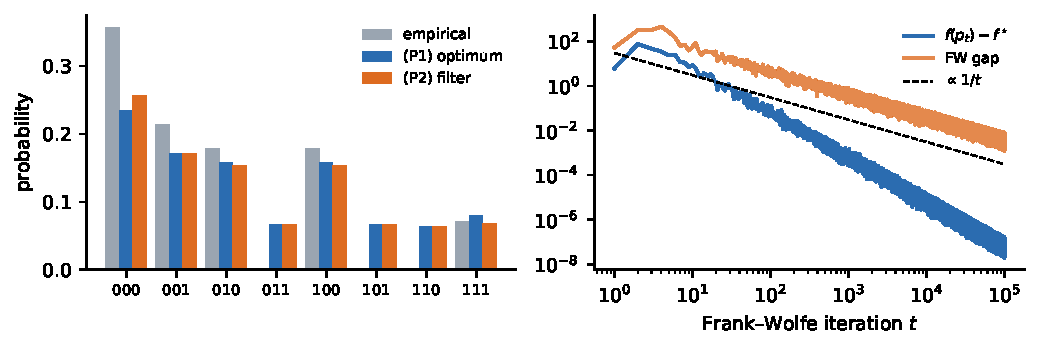
\includegraphics[width=\linewidth]{figures/fig_n3.pdf}
\caption{$n=3$. Left: empirical distribution, exact optimum of~\eqref{eq:p1} ($\mu=50$), and the closed-form filter~\eqref{eq:p2} at matched unobserved mass. Right: vanilla FW on~\eqref{eq:p1} from the uniform start. The suboptimality decays faster than $1/t$; the FW gap is a loose certificate.}
\label{fig:n3}
\end{figure}

\subsection{A sparse problem with a certified global optimum ($n=20$)}\label{sec:exp-n20}

Following the original notebook, we draw $m=90$ strings around three centres in $\{0,1\}^{20}$ with flip probabilities $0.045$, $0.055$ and $0.065$, giving $55$ distinct strings. We use $\lambda=5\times10^7$ ($\mu=95.4$). We solve~\eqref{eq:p1} exactly on the radius-2 Hamming ball around the data ($7381$ states). We then certify optimality over all $2^{20}$ states: by the argument in \cref{sec:p1}, only the outer boundary of the ball can have negative gradients, and we include it in the FW gap. The result is the global optimum to gap $2.3\times10^{-7}$ (\cref{tab:n20}). Solving on the radius-1 ball gives the identical solution. The optimum has $62$ support points, the $55$ observed strings plus $7$ neighbours at distance~1, carrying $0.26\%$ of the mass. This confirms the obstacle-problem picture of \cref{prop:support}. The bound (d) evaluates to $294$, which is loose because here the smoothness term is large ($2\mu p^\top Lp=76$ against $m=90$), but still far below $2^{20}$. The sparse FCFW with $T=2$, $R=3000$ from the notebook finds $56$ support points and comes within $3.1\times10^{-3}$ of the optimum ($\ell_1$ distance $0.0064$) in about one second.

\begin{table}[t]
\centering
\caption{$n=20$, $m=90$, $\mu=95.4$. The exact optimum is certified over all $2^{20}$ strings.}\label{tab:n20}
\begin{tabular}{lcccc}
\toprule
 & objective & support & unobserved mass & global FW gap\\
\midrule
empirical $\hp$ & $410.5604$ & $55$ & $0$ & --\\
sparse FCFW ($T{=}2$, $R{=}3000$) & $368.4010$ & $56$ & $0.0006$ & --\\
exact (radius-2 ball + boundary) & $368.3978$ & $62$ & $0.0026$ & $2.3\times10^{-7}$\\
\bottomrule
\end{tabular}
\end{table}

\begin{table}[t]
\centering
\caption{Clock invariance (\cref{prop:clock}) on the $n=20$ problem. In every run the support never changes. With the reset clock, $(T,R)$ and $(1,TR)$ differ; with the continuous clock they coincide exactly.}\label{tab:clock}
\begin{tabular}{cccccc}
\toprule
clock & $(T,R)$ & $f$ at $(T,R)$ & $f$ at $(1,TR)$ & $\Delta f$ & $\ell_1$ distance\\
\midrule
reset & $(8,40)$ & $497.12$ & $369.33$ & $127.79$ & $0.854$\\
reset & $(5,60)$ & $395.60$ & $369.07$ & $26.52$ & $0.521$\\
continuous & $(8,40)$ & $369.33$ & $369.33$ & $0$ & $0$\\
continuous & $(5,60)$ & $369.07$ & $369.07$ & $0$ & $0$\\
\bottomrule
\end{tabular}
\end{table}

\paragraph{Where does P2 put its mass?}
On the same data, the closed-form filter is strictly positive everywhere, as \cref{thm:p2} predicts. The mass on observed strings is $86\%$, $39\%$ and $6\%$ for $\mu=0.01$, $0.1$ and $1$; the rest spreads outward in Hamming shells. The parameter $\mu$ thus interpolates continuously between the empirical distribution and the uniform one.

\subsection{Generalisation and the checksum counterexample}\label{sec:exp-gen}

We compare the estimators at $n=10$, where every quantity can be computed exactly. The \emph{clustered} target is an equal mixture of four product distributions around random centres, each bit flipped with probability $0.1$. This target is smooth in Hamming distance. The \emph{checksum} target is the same mixture conditioned on even parity, which is a hard constraint that Hamming smoothing violates. For each target we draw $m\in\{30,100,300,1000\}$ samples over $10$ seeds.

The estimators are:
\begin{itemize}
\item the empirical distribution;
\item add-$\alpha$ (uniform pseudo-counts);
\item the heat / Aitchison--Aitken kernel;
\item the Tikhonov filter~\eqref{eq:p2};
\item penalised maximum likelihood~\eqref{eq:p1};
\item the learned positive isotropic filter of \cref{sec:filters} (LOO-EM), which has no hyperparameter.
\end{itemize}
To compare like with like, add-$\alpha$, heat and Tikhonov are tuned by the same criterion the learned filter optimises: full-data leave-one-out log-likelihood. Their grids include zero smoothing ($\alpha=0$, $\theta=0$, $\mu=0$). Zero smoothing is in fact never selected, and neither is the learned filter's identity endpoint $w_0=1$: without repeated strings both have leave-one-out likelihood $-\infty$. P1 has no closed-form leave-one-out score. Rather than refitting it $m$ times, we tune it on a $20\%$ validation split with the quadratic score $\|q\|_2^2-\frac{2}{|V|}\sum_{x\in V}q(x)$, a proper scoring rule~\cite{gneiting2007scoring}, and then refit on all $m$ samples. \Cref{tab:gen} and \cref{fig:gen} report the total-variation distance to the truth. Since all estimators see the same samples in each seed, we also report paired differences.

\begin{table}[t]
\centering
\caption{Total variation to the true distribution at $n=10$, given as mean (standard error $\times10^3$) over 10 seeds. Last column: mean mass on odd-parity strings for the checksum target at $m=100$, and the fraction of runs with $\mathrm{KL}(p\,\|\,q)<\infty$ for the clustered target at $m=1000$. Bold marks the best mean in each column.}\label{tab:gen}
\footnotesize
\setlength{\tabcolsep}{3pt}
\begin{tabular}{lccccccccc}
\toprule
& \multicolumn{4}{c}{clustered} & \multicolumn{4}{c}{checksum} & \\
\cmidrule(lr){2-5}\cmidrule(lr){6-9}
estimator & $m{=}30$ & $100$ & $300$ & $1000$ & $30$ & $100$ & $300$ & $1000$ & invalid / KL fin.\\
\midrule
empirical & .611(10) & .421(12) & .310(5) & .185(4) & .502(16) & .344(12) & .239(6) & \textbf{.136}(4) & 0 / 0.0\\
add-$\alpha$ & .562(12) & .439(17) & .327(3) & .183(3) & .553(8) & .364(10) & .275(14) & .162(5) & .115 / 1.0\\
heat (A--A) & \textbf{.403}(14) & \textbf{.284}(10) & \textbf{.238}(4) & \textbf{.164}(4) & .585(6) & .460(12) & .342(6) & .207(22) & .326 / 1.0\\
Tikhonov (P2) & .417(16) & .290(9) & .246(6) & .168(4) & .552(10) & .426(12) & .331(10) & .206(8) & .270 / 1.0\\
pen.\ MLE (P1) & .546(16) & .421(11) & .333(12) & .188(4) & .580(23) & .353(12) & .256(9) & .147(5) & .001 / 0.0\\
learned isotropic & .417(14) & .288(10) & \textbf{.238}(4) & .168(4) & \textbf{.382}(12) & \textbf{.269}(11) & \textbf{.210}(8) & \textbf{.136}(3) & 0 / 0.9\\
\bottomrule
\end{tabular}
\end{table}

\begin{figure}[t]
\centering
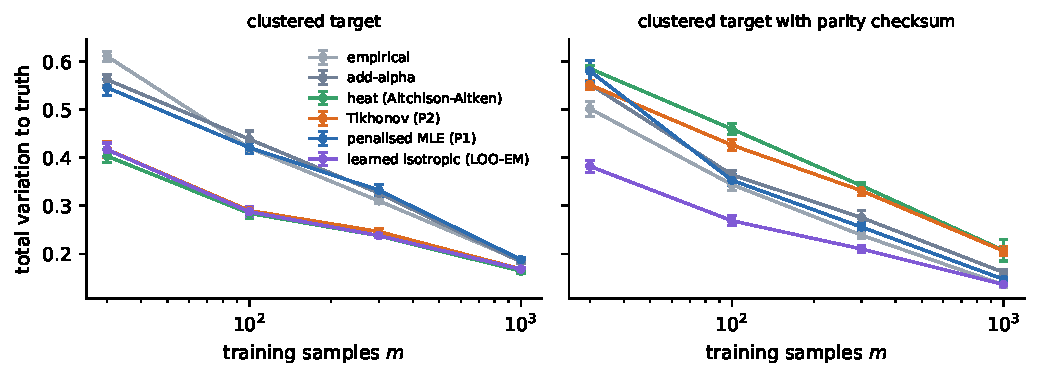
\includegraphics[width=\linewidth]{figures/fig_generalisation.pdf}
\caption{Total variation to the truth at $n=10$ (mean $\pm$ s.e., 10 seeds). On the smooth target, heat, Tikhonov and the learned filter are close to each other and well below the empirical distribution, while P1 barely improves on it. On the checksum target, the Hamming smoothers lose to the empirical distribution, and only the learned isotropic filter improves on it.}\label{fig:gen}
\end{figure}

\paragraph{Smooth target.}
Heat, Tikhonov and the learned filter all beat the empirical distribution and add-$\alpha$ at every $m$. The gain is largest at small $m$: at $m=30$, TV drops from $0.61$ to $0.40$--$0.42$. Among the three, the one-parameter heat kernel is as good as or slightly better than the learned filter. The paired difference (learned minus heat) is $+0.014\pm0.004$ at $m=30$ and $+0.004\pm0.001$ at $m=1000$, and within two standard errors of zero at $m=100$ and $300$. Against Tikhonov, the learned filter is within one standard error at $m=30$, $100$ and $1000$, and better by $0.008\pm0.003$ at $m=300$. On a target that really is Hamming-smooth, then, learning all $n+1$ shell weights buys nothing over tuning a single bandwidth by the same criterion, and costs a little variance at small $m$.

\paragraph{Penalised likelihood barely smooths here.}
P1 barely improves on the empirical distribution, and it has infinite KL in every run. This is consistent with \cref{prop:support}. In the runs we inspected ($m=100$ and $1000$), the support of the P1 optimum stays exactly equal to the set of distinct observed strings across the whole useful range of $\mu$. So in this regime P1 only \emph{reweights} the observed strings: it compresses the frequent ones and lifts the rare ones, but it does not move mass onto unseen strings, which is where most of the error lies. This is a property of the regime, not a general law. With few distinct strings and strong smoothing, P1 does spread mass (\cref{sec:exp-small}; the $n=1$ example in \cref{sec:p1}). Here larger $\mu$ only hurts, and validation drives $\mu\to0$ at large $m$. The cause is the likelihood term, which rewards mass on the data and gives no direct reward for mass elsewhere. The $\ell_2$ data term of P2 has no such effect.

\paragraph{The checksum counterexample.}
On the parity-constrained target, the Hamming smoothers lose to the empirical distribution at every $m$. Part of this is structural. Any heat kernel with $\theta>0$ leaks the mass $\Pr[\text{odd number of flips}]=\tfrac12\bigl(1-(1-2\theta)^{n}\bigr)$, which is already $4.8\%$ at the smallest positive grid value $\theta=0.005$. Leave-one-out selection makes this worse, not better: it favours $\theta\approx0.1$ at $m=30$, and heat and Tikhonov then put $27$--$45\%$ of their mass on invalid strings at $m\le100$.

The learned isotropic filter is the exception. It places \emph{exactly zero} mass on invalid strings. It beats heat and Tikhonov by $0.07$--$0.20$ in TV in every seed at every $m$, and it beats the empirical distribution in every seed for $m\le300$, tying it at $m=1000$. Its weights show why. For one seed at $m=100$, EM returns $w_0=0.74$, $w_2=0.26$ and $w_d=0$ otherwise. All pairwise distances within the data are even, so the leave-one-out likelihood puts all weight on even shells, and ``flip exactly two bits'' preserves parity. Isotropic does not mean Hamming-local. The positive isotropic class of \cref{thm:isotropic} is rich enough to express some hard constraints, while remaining exactly samplable in $O(n)$. The price is that zero weight on some shells can leave valid strings with zero mass, so its KL is not always finite at small $m$.


\subsection{Exact sampling at $n=100$}\label{sec:exp-large}

With $m=50$ random training strings in $\{0,1\}^{100}$ and $\mu=0.05$, the sampler of \cref{cor:sampler} draws $2\times10^5$ samples in $0.24$\,s. The empirical law of the number of flipped bits matches the exact law $\binom nd k_\mu(d)$ from~\eqref{eq:kernel} to total variation $0.005$ (\cref{fig:large}), which is at sampling-noise level. Exact density evaluation takes about $6\,\mu$s per query. At $n=10$ we also checked the sampler against the dense filter: its TV distance to the exact distribution matches that of an i.i.d.\ sample from the exact distribution at $10^4$, $10^5$ and $10^6$ draws.

\begin{figure}[t]
\centering
\begin{minipage}{0.48\linewidth}
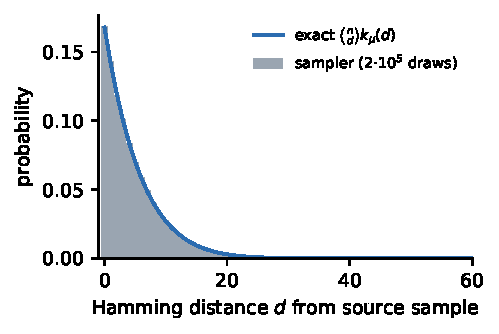
\includegraphics[width=\linewidth]{figures/fig_large_n.pdf}
\caption{$n=100$: law of the number of bits flipped by the Tikhonov sampler, empirical versus exact.}\label{fig:large}
\end{minipage}\hfill
\begin{minipage}{0.48\linewidth}
\small
\textbf{Identities verified numerically} ($n\le10$, $\mu\in\{0.01,1,100\}$):
$|\E(p)-2^{1-n}p^\top Lp|\le10^{-21}$; Walsh basis diagonalises $L$ exactly; $\min K_\mu>0$; column sums of $K_\mu$ equal $1$ to $10^{-13}$; the closed-form kernel~\eqref{eq:kernel} matches $(I+\mu L)^{-1}$ to relative error $\le2\times10^{-12}$; the Gauss--Jacobi formula matches the Krawtchouk expansion to $\le2\times10^{-13}$ for $\mu\in[10^{-3},10^3]$.
\end{minipage}
\end{figure}

\subsection{The filter zoo}\label{sec:exp-filters}

\Cref{fig:filters} shows five level filters at $n=20$ alongside their shell weights $w_d$. Noise, heat and Tikhonov have $w\ge0$ up to rounding. Band-limiting at $b=2$ ($\min w_d=-1.59$) and the Gaussian $e^{-k^2/8}$ ($\min w_d=-0.48$) have negative weights, so they do not preserve positivity. Band-limiting the empirical distribution of $30$ random samples at $n=10$ produces an average of $15\%$ negative mass, with a maximum of $20\%$ over $20$ draws.

\begin{figure}[t]
\centering
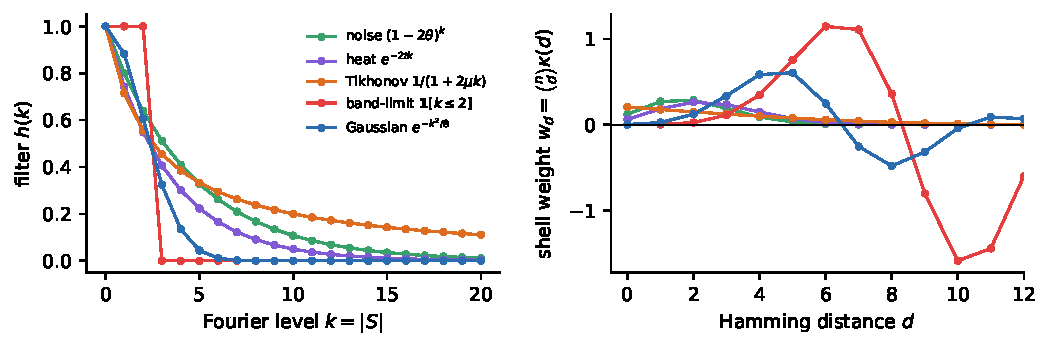
\includegraphics[width=\linewidth]{figures/fig_filters.pdf}
\caption{Left: isotropic filters $h(k)$ at $n=20$. Right: the corresponding shell weights $w_d=\binom nd\kappa_h(d)$ (\cref{thm:isotropic}). A filter maps every distribution to a distribution if and only if all $w_d\ge0$. Hard band-limiting and this Gaussian fail, even though both are ``low-pass''.}
\label{fig:filters}
\end{figure}

% ------------------------------------------------------------------------------
\section{Discussion and limitations}

\paragraph{The metric is the model.}
Everything here is relative to the Hamming graph. Smoothness in raw Hamming distance is the wrong bias when the encoding is not semantic, for example with checksums, Gray versus binary codes, or permuted fields. The graph Laplacian template carries over to any other graph on $\B$, but the Walsh diagonalisation, and with it the $O(n)$ samplers, are special to the hypercube and its Cayley-graph relatives. For general groups, \cite{belis2026spectral} discusses the corresponding Fourier transforms.

\paragraph{Scope.}
All experiments are synthetic and small enough for exact verification. We compare estimators only by total variation and KL divergence to a known ground truth. We have not run any quantum experiment. \Cref{sec:quantum} is an argument about where an advantage could live, not evidence that one exists.

\paragraph{What the optimisation view bought.}
Starting from an objective rather than a filter exposed the scaling $\mu=\lambda2^{1-n}$ and the obstacle-problem structure of the likelihood-based estimator. It also gave a natural reason why the filter's output must be a distribution, which then led to the noise-channel characterisation. The step-size-clock issue is a reminder that empirical invariances, here ``same support, same budget, same answer'', are cheap and effective unit tests for optimisers.

% ------------------------------------------------------------------------------
\section{Conclusion}

Smoothing a bitstring distribution with the hypercube Dirichlet energy leads, through an $\ell_2$ data term, to the Walsh filter $1/(1+2\mu|S|)$. This filter never violates positivity: it is a random number of random bit flips, so it can be sampled and evaluated classically at any scale. More generally, a spectral filter maps every distribution to a distribution exactly when it is the characteristic function of a noise distribution. In the isotropic case, all such filters are mixtures of ``flip $d$ bits'' channels and can be learned by a concave likelihood. Any genuine quantum role in this example must therefore come from noise that is hard to sample yet still useful for smoothing, or from amplitude-level models that leave the class of convolutional smoothers altogether. We think making that distinction explicit is a useful step towards the ``why quantum?'' question that Belis et al.\ rightly put first.

\paragraph{Acknowledgements.}
This paper grew out of a blog post working through~\cite{belis2026spectral}. Parts of the analysis, code and text were drafted with the assistance of an AI model (Claude, Anthropic) and checked by the author.

\bibliographystyle{unsrtnat}
\bibliography{refs}

% ------------------------------------------------------------------------------
\appendix
\section{Implementation details}

\paragraph{Solvers.}
Dense problems ($n\le10$) use the fast Walsh--Hadamard transform for all filters and a vectorised Laplacian. The exact solver for~\eqref{eq:p1} stops when the FW gap falls below $10^{-7}m$, or after $4000$ iterations, in \cref{sec:exp-gen}; in \cref{sec:exp-n20} the target gap is $10^{-10}m$, and the run reached $2.3\times10^{-7}$ after $10^5$ iterations. On a restricted state set $B$, the Laplacian is $(L_Bp)_x=np_x-\sum_{y\sim x,y\in B}p_y$, which is exact for vectors supported in $B$. The global certificate adds the boundary strings $y\notin B$ with gradient $-2\mu\sum_{x\sim y}p_x$ and the value $0$ for all other strings.

\paragraph{Hyperparameters in \cref{sec:exp-gen}.}
Add-$\alpha$: $\alpha\in\{0\}\cup\{10^{-3},\dots,10\}$ (9 log-spaced values plus $0$). Heat: flip probability $\theta\in\{0\}\cup[0.005,0.35]$ (15 values plus $0$). Tikhonov: $\mu\in\{0\}\cup[10^{-3},10^{1.5}]$ (15 log-spaced values plus $0$). These three are selected by full-data leave-one-out log-likelihood, computed in closed form from the pairwise distances (add-$\alpha$: $(c_{x_j}-1+\alpha)/(m-1+2^n\alpha)$). P1: $\mu=a\,m^2/n$ with $a\in[10^{-6},10^2]$ (9 log-spaced values); this scaling balances $c_x/p_x\approx m$ against $2\mu(Lp)_x\sim\mu n/m$. P1 is selected by the quadratic score on a $20\%$ validation split (at least 5 samples), followed by a refit on all data.

\paragraph{Reproducibility.}
\texttt{python run\_experiments.py [e1 \dots e6]} regenerates every number and figure. E1--E3, E5 and E6 run in about two minutes; E4 takes longer, dominated by the~\eqref{eq:p1} grid.

\end{document}
